\documentclass[11pt, oneside]{article}   	% use "amsart" instead of "article" for AMSLaTeX format
\usepackage[margin=1in]{geometry}                		% See geometry.pdf to learn the layout options. There are lots.
\geometry{letterpaper}                   		% ... or a4paper or a5paper or ... 
%\geometry{landscape}                		% Activate for rotated page geometry
%\usepackage[parfill]{parskip}    		% Activate to begin paragraphs with an empty line rather than an indent
\usepackage{graphicx}				% Use pdf, png, jpg, or eps§ with pdflatex; use eps in DVI mode
								% TeX will automatically convert eps --> pdf in pdflatex		
\usepackage{amssymb}
\usepackage{awesomebox}
%SetFonts

%SetFonts

\usepackage{amsmath}
\DeclareMathOperator{\plainmod}{\text{ mod }}
\let\emptyset\varnothing

\newcommand{\reals}{\mathbb{R}}
\newcommand{\realsText}{$\mathbb{R}$}
\newcommand{\ints}{\mathbb{Z}}
\newcommand{\intsText}{$\mathbb{Z}$}

\title{Homework 8}
\author{Discrete Structures 2}
\date{due: 4 May 2023, 8:00am}							% Activate to display a given date or no date

\begin{document}
\maketitle
%\section{}
%\subsection{}

Your task for this homework will be to answer the following questions without using any calculating resources. 
Your responses should be submitted via blackboard by the due date above as a PDF (submissions in any other format will be returned to the user and a resubmissions will be requested). 
You are free to use whatever tools you would like to generate the response document: 
scanned hand-written paper, 
tablet generated hand-written, 
microsoft word (with this option, please use the equation editor to correctly format your responses), 
\LaTeX, etc.
Your TA, IA, and Instructor are available to help during their designated office hours or via email 
(note that emails sent during non-business hours may not be responded to until the next working day). 

%\importantbox{
%\textbf{Note:} all of these questions are on topics from chapters 5; thus you will only be proving by induction in this homework assignment. 
%}
\begin{enumerate}
% 6.18
\item Prove the transitivity of $O(\cdot)$ (we described this property in class without justification): \\
if $f(n)=O(g(n))$ and $g(n)=O(h(n))$, then $f(n)=O(h(n))$.
% 6.21
\item Prove if $p(n) = \sum_{i=0}^{k} a_i n^k$ is a polynomial, then $p(n) = O(n^k)$.

%6.102
\item Consider the following recurrence relation: 
\[
C(1) = 0 \text{   and  } C(n) = 2C\left( \frac{n}{2} \right) + n - 1.
\]
Prove that $C(n) = n \log n - n + 1$ by induction. 
(For ease, we’ll assume that n is a power
of two.)

%6.107/108
\item (A true story, inspired by Michael Eisen’s 2011 blog post ``Amazon’s \$23,698,655.93 book about flies''.) 
Two copies of an out-of-print book were listed online by Seller A and Seller B. Their prices were over \$1,000,000 each --- 
and the next day, both prices were over \$2,000,000, and they kept going up. 
By watching the prices over several days, it became clear that the two sellers were using algorithms to set their prices in response to each other. 
Let $a_n$ and $b_n$ be the prices offered on day $n$ by Seller $A$ and Seller $B$, respectively. 
The prices were set by two (badly conceived) algorithms such that $a_n = \alpha \cdot b_{n-1}$ and $b_n = \beta \cdot a_n$ where $\alpha = 0.9983$ and $\beta = 1.27059$.
\begin{enumerate}
\item Suppose that $b_0 = 1$. Find closed-form formulas for $a_n$ and $b_n$. Prove your answer.
\item State a necessary and sufficient condition on $\alpha, \beta, and b_0$ such that $a_n = \Theta(1)$ and \\$b_n = \Theta(1)$.
\end{enumerate}

%6.130
\item 
\label{q:towers}
The \emph{Towers of Hanoi} is the following classic puzzle. 
There are three posts (the ``towers''); 
post $A$ starts with $n$ concentric discs stacked in order of their radius (smallest radius at the top, largest radius at the bottom). 
We must move all the discs to post $B$, never placing a disc of larger radius on top of a disc of smaller radius. 
The easiest way to solve this puzzle is with recursion. 
(See Figure~\ref{fig:towers}) 
The total number of moves made satisfies $T(n) = 2T(n-1) + 1$ and $T(1) = 1$. 
Prove that $T(n) = 2^n - 1$.

\begin{figure}
\begin{center}
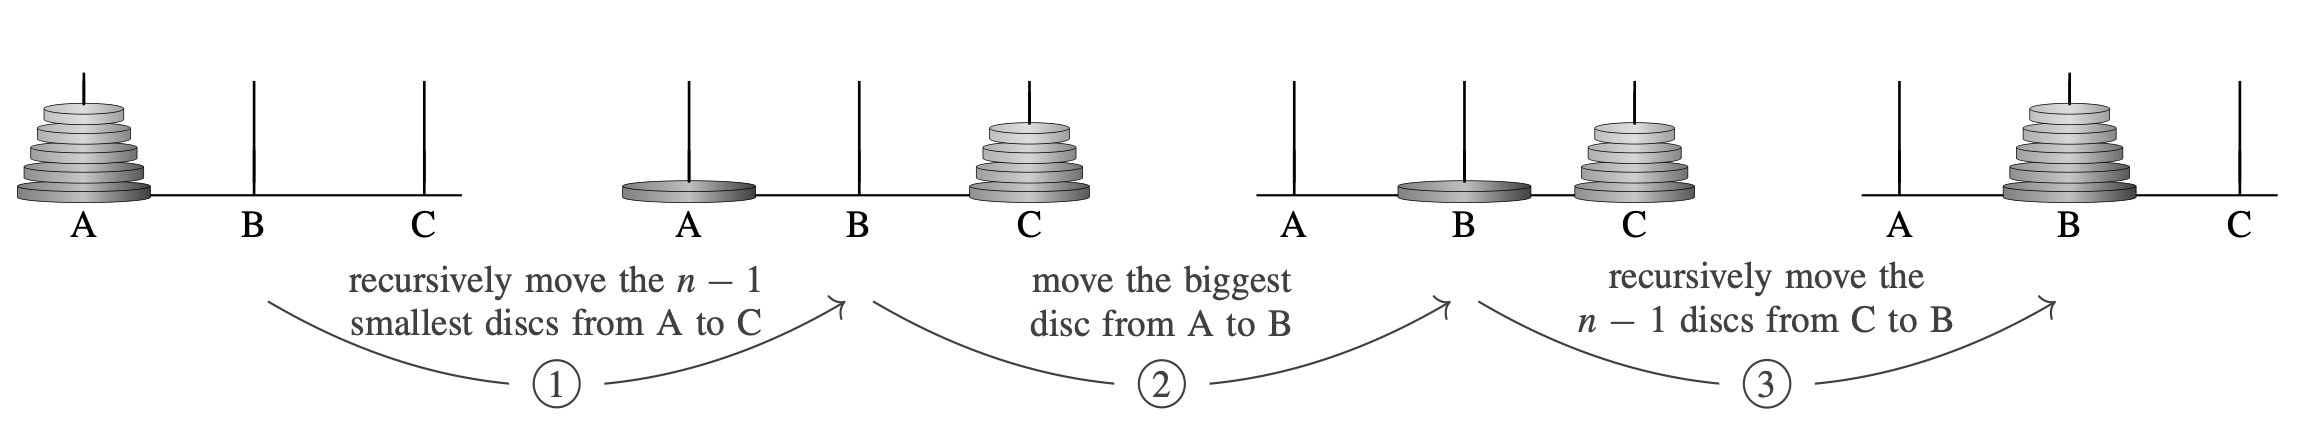
\includegraphics[width=\textwidth]{towers}
\caption{Pictorial of Towers of Hanoi for Question~\ref{q:towers}}
\label{fig:towers}
\end{center}
\end{figure}


\item The following recurrence relations follow the form of the summary formula from the slides. Solve each. Assume $T(1) = 1$.
\begin{enumerate}
\item $T(n)=4T\left(\frac{n}{3}\right)+n^2$ %6.109
\item $T(n)=3T\left(\frac{n}{3}\right)+n$ %6.112
\item $T(n)=2T\left(\frac{n}{4}\right)+1$ %6.114
\item $T(n)=2T\left(\frac{n}{4}\right)+n^2$ %6.119
\item $T(n)=4T\left(\frac{n}{2}\right)+n$ %6.122

\end{enumerate}
\end{enumerate}
\end{document}